\chapter{Learning framework}\label{learning_framework}
    In this chapter, I briefly describe the framework that can be used to learn how to classify the vertices of the Wikipedia multilingual graph described in chapter \ref{wikipedia_multilingual_graph}.
    
    The framework makes a user's life easier by providing him/her with some utilities for dealing with features, labels and curriculum associated with the Wikipedia multilingual graph: one does not need to write a lot of code and only has to follow the simple flow of control describe in next sections. Most importantly, all the functions described here are completely integrated with the formats described in chapter \ref{wikipedia_multilingual_graph}: this means that a users does not have to worry about the conversion between different interfaces.
    \section{Features}\label{features}
        In this setting, a feature is a measurable property or characteristic of a vertex of the multilingual graph. The graph itself --- i.e., the set of vertices and edges --- is not considered to be a feature. In fact, it represents the structure of the domain on which data lies. Refer to section \ref{domainstructure_datadomain} --- and, in particular, to figure \ref{data_on_domain} --- for more details about the difference between domain structure and data on a domain.
        
        In general, once the domain structure is ready --- i.e., when the multilingual graph has been built --- the framework allows users to add data on the domain --- i.e., vertex features. In particular, the framework provides users with:
        \begin{itemize}
            \item A method for loading arbitrary features.
            \item A method for computing word embeddings of page titles or summaries. These embeddings can be used as vertex features.
        \end{itemize}
        Adding vertex features is not a mandatory operation, and it has both advantages and disadvantages: a compromise must be found. However, features cannot be added to a subset of the vertices: every vertex must have the same number of features. Moreover, in order to be meaningful and useful, values on different vertices should come from the same distribution.
        \subsection{Strengths and weaknesses of features}
            Choosing discriminating and independent features is a crucial step for effective learning algorithms. Indeed, the underlying graph is not always informative enough: while one can reach a high accuracy in classifying the vertices of a multilingual graph built with well developed Wikipedia versions, the structure of the graph may not be sufficient and adequate when dealing with minor wikis.
        
            It is not mandatory to use features, though. Indeed, one can use the learning framework for classifying vertices of the multilingual graph even using only structure information. In general, having data on the domain has both advantages and disadvantages:
            \begin{itemize}
                \item In general, there are two possible --- and almost opposite --- reasons a model may not perform well: high bias and high variance. As described in section \ref{biasvariance}, bias refers to the systematic error that the learning algorithm is expected to make, variance captures how much the algorithm's predictions are spread out from their average value. On one hand, high bias problems would probably very well benefit from more features. On the other hand, a way to address high variance problems is by reducing the number of features. In general, better data does not mean more data; as a matter of fact, sometimes it might mean less: \textquote{the selection of relevant features, and the elimination of irrelevant ones, is one of the central problems in machine learning} \cite{Blum}.
                \item The learning framework can work with graph neural networks (see sections \ref{spectralgeometriclearning} and \ref{experiments_gcn}). It is relatively easy to learn node embeddings for fixed graphs --- i.e., graphs that do not change over time --- with these algorithms: they work well even if no features are used. However, as pointed out by \citeauthor{Kipf} (authors of \cite{Kipf} and some of the pioneers of geometric deep learning), when dealing with dynamic graphs, one can make predictions on new nodes only if their feature vectors come from a similar underlying distribution\footnote{\url{http://tkipf.github.io/graph-convolutional-networks/}.}. In fact, if one uses no features, the prediction would mostly be just random.
                \item When dealing with large graphs, as in this setting, more practical problems might arise: memory requirements quickly increase. Moreover, there could be a severe performance drop, especially if the chosen machine learning model does not scale well. In general, one must deal with the computational resources he/she has, and find a good compromise between size of the multilingual graph, number of features, performance and memory usage.
            \end{itemize}
        \subsection{Load features}\label{load_features}
            The framework includes a useful function that allows to automatically load arbitrary feature vectors stored in a file. In this way, a user can obtain data from independent sources, save them on disk\footnote{Computing features for a large number of vertices is usually computationally expensive. Therefore, it does not make sense to compute the same thing more than once: data should be persistently saved for future reuse.} and load them every time the learning framework is run.
            
            The function works with CSV files\footnote{Text files that uses comma to separate values. Sometimes, the term CSV denotes some closely related delimiter-separated formats that use different field delimiters (such as tab).}: this format is best used for representing sets of records in which each record has an identical list of fields.
            
            Here is a summary of what the function does and a complete description of parameters and outputs. The specific format of the CSV file will be described afterwards.
            \begin{independentfunctiondoc}{load\_features}{graph, path}
                \begin{functiondescription}
                    Load numerical vertex features from a CSV file.
                \end{functiondescription}
                
                \begin{functionparameters}
                    \item[graph] \monospace{graph\_tool.Graph}
                    
                    Wikipedia graph.
                    
                    It can represent either a multilingual or a monolingual Wikipedia graph. Refer to section \ref{categorygraphbuilder}, \ref{articlegraphbuilder} and \ref{multilingualbuilder} for checking how to build such specific graphs.
                    \item[path] string
                    
                    File path where the CSV file will be loaded.
                \end{functionparameters}
                
                \begin{functionoutput}
                    \monospace{graph\_tool.VertexPropertyMap} object (see \url{https://graph-tool.skewed.de/static/doc/graph_tool.html\#graph_tool.VertexPropertyMap}), with associated value type \inlinecode{vector<double>}.
                    
                    It is a class that provides a mapping from vertices to arbitrary properties. It can be thought of as a way of associating vectors of doubles to the vertices of the graph.
                    
                    Compared to vertex internal properties --- such as IDs and names, see sections \ref{categorygraphbuilder}, \ref{articlegraphbuilder} and \ref{multilingualbuilder}) --- the result of this function is external property: this means that it is not internalized by including it in the graph's dictionary-like attributes, and it does not need a name.
                \end{functionoutput}
            \end{independentfunctiondoc}
            \subsubsection{CSV file format}
                The CSV file from which features are loaded is formatted according to some standard basic rules:
                \begin{itemize}
                    \item It has no \textquote{header}.
                    \item Each line consists of a vertex index (a positive integer value) followed by one or more rational numbers (double values). These numbers represent the feature vector associated to the vertex.
                    \item Each line consists of exactly the same number of fields.
                    \item Values are separated by commas and are not quoted.
                    \item There are no leading and trailing spaces and/or tabs in any field.
                    \item The decimal separator is the standard period/full stop.
                \end{itemize}
                
                There is also a rule that applies to this specific setting: a file must contain one and only one line for each vertex. This means that the CSV file must have as many lines as the number of vertices in the Wikipedia graph, and that there must be exactly one occurrence of each vertex index. The specific order of lines does not matter.
                
                Here is a practical example. Suppose that \inlinecode{graph} is an object of type \monospace{graph\_tool.Graph}. This graph has exactly three nodes (with index \(0\), \(1\) and \(2\)). Also, suppose that the content of the CSV file \textquote{input.csv} is
                \begin{lstlisting}
2,4.5,2.7568,3.2,17
0,-0.1,20,4.2,54,2.543
1,6.77,299,455,1
                \end{lstlisting}
                Then, the following code loads three feature vectors (one for each node) with four values each, and obtain the vector associated with the second vertex:
                \begin{example}
// load features
features = load_features(graph, "input.csv")
// get the feature vector of the second vertex
v1 = graph.vertex(1)
v1_features = features[v1] // [6.77, 299, 455, 1]
                \end{example}
        \subsection{Multilingual word embeddings}
            While loading arbitrary feature vectors is very flexible, a user may want to have a ready-to-use function that is able to compute some useful features in order to try to use the learning framework. Moreover, computing vertex features for multilingual graphs is not easy, especially because they are supposed to come from the same underlying distribution.
            
            The framework includes a function that can build a numerical representation of the title or the summary of each page contained in the multilingual graph. It makes use of two open source libraries developed at Facebook:
            \begin{itemize}
                \item MUSE\footnote{\url{http://github.com/facebookresearch/MUSE}} \cite{Conneau}\cite{Lample} is library for multilingual word embeddings. In other words, it provides a mapping from a \textquote{concept space} to a \(300\)-dimensional vector space: the more similar the meaning of two words in different languages is, the closer the related mappings in the vector space are.
                \item FastText\footnote{\url{http://fasttext.cc/}.} is a library that allows users to learn text representations. Moreover, it provides methods for reducing embeddings in size to fit low resource settings. Finally, it also provides aligned word vectors for 44 languages based on the pre-trained vectors computed on Wikipedia\footnote{\url{http://fasttext.cc/docs/en/aligned-vectors.html}.} \cite{Joulin}\cite{Bojanowski}: this helps to reduce the computation time by a big factor.
            \end{itemize}
            
            When the Wikipedia multilingual graph is based on one of the 44 pre-trained languages provided by FastText, the function simply downloads the files and extracts data from them. Instead, when users build the graph using some minor Wikipedia versions, the function build the embeddings using the MUSE library. Once vectors are obtained, FastText is used to combine them and get a single embedding for either the page title or summary.
            
            Here is a summary of what the function does and a complete description of parameters and outputs. For an in-depth explanation of parameters and output, refer to the \monospace{load\_features} function (presented in section \ref{load_features}), which shares many details with the function described below.
            \begin{independentfunctiondoc}{multilingual\_word\_embeddings}{graph, mode}
                \begin{functiondescription}
                    Build a numerical representation (a \(300\)-dimensional vector) of the title or the summary of each page contained in the multilingual graph.
                    
                    The function relies on the open source MUSE and FastText libraries.
                \end{functiondescription}
                
                \begin{functionparameters}
                    \item[graph] \monospace{graph\_tool.Graph}
                    
                    Wikipedia graph.
                    
                    It can represent either a multilingual or a monolingual Wikipedia graph. Refer to section \ref{categorygraphbuilder}, \ref{articlegraphbuilder} and \ref{multilingualbuilder} for checking how to build such specific graphs.
                    \item[mode] \{\inlinecode{"title"}, \inlinecode{"summary"}\}
                    
                    Text to be used to create the embeddings:
                    \begin{enumerate}
                        \item \inlinecode{"title"}: use only the words in page titles.
                        \item \inlinecode{"summary"}: use only the words in page summaries.
                    \end{enumerate}
                \end{functionparameters}
                
                \begin{functionoutput}
                    \monospace{graph\_tool.VertexPropertyMap} object, with associated value type \inlinecode{vector<double>}.
                    
                    This object provides a mapping from vertices of the graph to vectors of doubles. It is an external property: it is not memorized together with the graph and it does not need a name.
                \end{functionoutput}
            \end{independentfunctiondoc}
    \section{Labels}\label{labels}
        As described in sections \ref{classification} and \ref{semi_supervised}, (semi-)supervised classification algorithms attempt to estimate the mapping function from the inputs to categorical outputs by using several input-output pairs. Outputs are often called labels or categories.
        
        In this setting, inputs are given by both the graph --- i.e., the domain structure --- and the features --- i.e., the data on domain (refer to section \ref{domainstructure_datadomain}). Hence, inputs can be represented by graph vertices.
        
        With regard to outputs, they can be of two types: \emph{hard} or \emph{soft} labels. The former is the class the model predicts, the latter represents the probability of data point belonging to each of the possible classes.
        
        Therefore, one needs a way to indicate which are the labeled vertices and the associated labels (either hard or soft). In general, once the multilingual graph has been built (see sections \ref{categorygraphbuilder}, \ref{articlegraphbuilder} and \ref{multilingualbuilder}), the framework provides users with some methods for dealing with labels:
        \begin{itemize}
            \item Two general functions allow to load, respectively, hard and soft labels. In this way, a user can start training a machine learning model using his/her own data.
            \item A function allows to use the labels provided by Negapedia. By using this method, a user can quickly get some labels to start testing the learning framework.
            \item A function for getting a list of the most informative vertices of the graph. It can be used to find out which are the vertices one should try to label before running the learning algorithm.
            \item A function for getting all the labels collected through the labelling platform described in chapter \ref{labelling_platform}.
        \end{itemize}
        
        Adding labels is strictly required if one wants to run the semi-supervised learning algorithm. Ideally, a user should label the most informative vertices (refer to section \ref{active_learning}) in order to propagate the information quickly. However, users do not need to add labels to each single graph vertex: only a small subset should be labeled. Indeed, semi-supervised methods do not require a lot of labeled training data. A good starting point is desirable, though --- i.e., one should try to have a high quality initial training set.
        \subsection{Load labels}
            The framework includes a couple of functions that allow to load arbitrary labels stored in a file. In this way, users can compute vertex labels using their own methods and sources, store them on a file and load them every time they need to use the learning framework.
            
            There are two types of labels the framework can deal with: \textquote{hard} and \textquote{soft} labels. According to \cite{Galstyan}:
            \begin{itemize}
                \item A hard label is a label assigned to a member of a class where membership is binary: either the element in question is a member of the class (has the label), or it is not.
                \item A soft label is one which has a probability attached to it. So the element is a member of the class in question with a certain probability. This implies that an element can have different membership scores related to each possible class.
            \end{itemize}
            In this specific setting (single-label classification problem), using hard labels corresponds to assigning a single categorical label to an input; using soft labels corresponds to assigning a probability distribution over the possible classes to an input.
            
            Both the functions presented below (one for hard labels and one for soft labels) work with CSV files: this means that data can be re-used also outside these specific settings.
            
            Here is a summary of what each function does and a complete description of parameters and outputs. The specific format of the CSV file will be described afterwards.
            \begin{independentfunctiondoc}{load\_hard\_labels}{graph, path}
                \begin{functiondescription}
                    Load \textquote{hard} labels to be assigned to graph vertices.
                \end{functiondescription}
                
                \begin{functionparameters}
                    \item[graph] \monospace{graph\_tool.Graph}
                    
                    Wikipedia graph.
                    
                    It can represent either a multilingual or a monolingual Wikipedia graph. Refer to section \ref{categorygraphbuilder}, \ref{articlegraphbuilder} and \ref{multilingualbuilder} for checking how to build such specific graphs.
                    \item[path] string
                    
                    File path where the CSV file will be loaded.
                \end{functionparameters}
                
                \begin{functionoutput}
                    \monospace{graph\_tool.VertexPropertyMap} object (see \url{https://graph-tool.skewed.de/static/doc/graph_tool.html\#graph_tool.VertexPropertyMap}), with associated value type \inlinecode{int}.
                    
                    This object provides a mapping from vertices of the graph to positive integers. These numbers represent the \textquote{hard} labels each vertex is associated with. The object is an external property: it is not memorized in the graph's dictionary-like attributes and it does not need a name.
                \end{functionoutput}
            \end{independentfunctiondoc}
            \begin{independentfunctiondoc}{load\_soft\_labels}{graph, path}
                \begin{functiondescription}
                    Load \textquote{soft} labels to be assigned to graph vertices.
                \end{functiondescription}
                
                \begin{functionparameters}
                    \item[graph] \monospace{graph\_tool.Graph}
                    
                    Wikipedia graph.
                    
                    It can represent either a multilingual or a monolingual Wikipedia graph.
                    \item[path] string
                    
                    File path where the CSV file will be loaded.
                \end{functionparameters}
                
                \begin{functionoutput}
                    \monospace{graph\_tool.VertexPropertyMap} object, with associated value type \inlinecode{vector<double>}.
                    
                    This object provides a mapping from vertices of the graph to vectors of doubles. These vectors represent the \textquote{soft} labels each vertex is associated with --- i.e., the probability distribution over the possible classes. The object is an external property: it is not memorized together with the graph and it does not need a name.
                \end{functionoutput}
            \end{independentfunctiondoc}
            \subsubsection{CSV file format}
                The CSV file from which labels (either \textquote{hard} or \textquote{soft}) are loaded is formatted according to some standard basic rules:
                \begin{itemize}
                    \item It has no \textquote{header}.
                    \item Each line consists of exactly the same number of fields.
                    \item Values are separated by commas and are not quoted.
                    \item There are no leading and trailing spaces and/or tabs in any field.
                    \item The decimal separator is the standard period/full stop.
                \end{itemize}
                With regard to the specific format required by \monospace{load\_hard\_labels} and \monospace{load\_soft\_labels} functions, each line of the file consists of a vertex index\footnote{Not to be confused with language IDs associated to each vertex of a Wikipedia multilingual graph.} (a positive integer value) followed by:
                \begin{itemize}
                    \item A single positive integer value representing a class, in case the user is loading hard labels.
                    \item A list of rational numbers (double values) representing a probability distribution over classes, in case the user user is loading soft labels.
                \end{itemize}
                When dealing with soft labels, each line must have the same number of fields: it corresponds to the number of possible classes a vertex can be assigned to. Moreover, all the values that follow the vertex index must sum up to 1 because they represent a probability distribution. When dealing with hard labels, the single value must be integer (strings and double values are not accepted) and greater than or equal to zero. Finally, there is a rule that applies to both files: they can contain up to one line for each graph vertex: there cannot be two lines referring the same vertex. The specific order of lines does not matter.
                
                Here is an example of a well-formatted CSV file containing soft labels:
                \begin{lstlisting}
3,0.2,0.3,0.5
6,0.1,0,0.9
5,0.6,0.3,0.1
                \end{lstlisting}
                The following code can load soft labels from an \textquote{input.csv} file with the content above. In order for the function to work, the graph has to have at least seven vertices.
                \begin{example}
// load labels
labels = load_soft_labels(graph, "input.csv")
// get the probability distribution of the fourth vertex
v3 = graph.vertex(3)
v3_labels = labels[v3] // [0.2, 0.3, 0.5]
                \end{example}
        \subsection{Negapedia labels}\label{negapedia_label_function}
            Having two functions for loading arbitrary labels is very flexible. However, a user may want to have a ready-to-use function that can be used for quickly getting some labels. In this way, the user can try out the framework without any prior knowledge on how to get or compute training labels.
            
            The framework includes a function that computes the labels of the vertices using the algorithm presented by \citeauthor{Bonetti} in \cite{Bonetti} and used by Negapedia to classify some Wikipedia pages\footnote{\url{http://github.com/ebonetti/wikiassignment}.} (for more details, refer to chapter \ref{negapedia} and, specifically, to section \ref{negapedia_algorithm}). This algorithm has been tuned and optimized on the English and Italian Wikipedia, and it still has problems on other wikis: labels provided by this algorithm cannot be always trusted but they provide a good starting point for training a machine learning model.
            
            Clearly, this function does not provide users with a way to specify which are the possible labels: one must accept the categorization system offered by Negapedia (more details about the categories used by Negapedia can be found in section \ref{negapedia_categories}; for updated data, check the categories page on the official Negapedia website\footnote{\url{http://en.negapedia.org/categories/}.}).
            
            Here is a summary of what the function does and a complete description of its parameters and outputs.
            \begin{independentfunctiondoc}{negapedia\_labels}{graph, type, min\_prob=0}
                \begin{functiondescription}
                    Compute the labels to be assigned to graph vertices using the results provided by Negapedia.
                    
                    The function relies on the open source library \monospace{wikiassignment} developed by \citeauthor{Bonetti} (\url{http://github.com/ebonetti/wikiassignment}).
                \end{functiondescription}
                
                \begin{functionparameters}
                    \item[graph] \monospace{graph\_tool.Graph}
                    
                    Wikipedia graph.
                    
                    It can represent either a multilingual or a monolingual Wikipedia graph.
                    \item[type] \{\inlinecode{"hard"}, \inlinecode{"soft"}\}
                    
                    Label type to be used:
                    \begin{enumerate}
                        \item \inlinecode{"hard"}: get hard labels out of Negapedia.
                        \item \inlinecode{"soft"}: get soft labels out of Negapedia.
                    \end{enumerate}
                    
                    Since the classification algorithm behind Negapedia computes a probability distribution over classes for each page, hard labels are computed by returning the index related to the largest value of the distribution.
                    
                    For example, if \inlinecode{type="hard"} then the hard label related to the \(\left[0.2,\ 0.5,\ 0.3\right]\) distribution is \(1\).
                    \item[min\_prob] float, default \inlinecode{0}
                    
                    Minimum value that the maximum of a probability distribution can have.
                    
                    The classification algorithm behind Negapedia computes a probability distribution over classes for each page. This parameter allows to keep only those distributions whose highest value is strictly greater than the parameter value itself.
                    
                    For example, if \inlinecode{min_prob=0.7} then the soft label \(\left[0.4,\ 0.3,\ 0.3\right]\) is discarded and \(\left[0.2,\ 0.05,\ 0.75\right]\) is kept.
                \end{functionparameters}
                
                \begin{functionoutput}
                    \monospace{graph\_tool.VertexPropertyMap} object. The associated value type depends on the value of the \normale{\emph{type}} \normalfont parameter:
                    \begin{enumerate}
                        \item If \inlinecode{type="hard"} then the associated value type is \inlinecode{int}.  The object thus represents a mapping from vertices to positive integers representing hard labels.
                        \item If \inlinecode{type="soft"} then the associated value type is \inlinecode{vector<double>}. The object thus represents a mapping from vertices to vectors of doubles. These vectors represent the probability distributions over classes of vertices.
                    \end{enumerate}
                    
                    The object is an external property: it is not memorized in the graph's dictionary-like attributes and it does not need a name.
                \end{functionoutput}
            \end{independentfunctiondoc}
            Since the algorithm behind Negapedia does not make use of the concept of multilingual graph, it might provide different labels for vertices that have been merged in the multilingual graph. When this is the case, the average of the different distributions is taken.
        \subsection{User-defined labels}
            As described in chapter \ref{labelling_platform}, I have developed a labelling platform that provides a graphical interface for labelling Wikipedia pages. Moreover, it offers a REST-based API to access data.
            
            A user that makes use of the labelling platform probably wants to gather labeled data that is stored in the platform database. For this reason, the framework offers a function that is able to automatically download labeled data data from the labelling platform database, and extracts labels to be assigned to vertices of the multilingual graph. This function simply wraps the REST-based API provided by the labelling platform and described in section \ref{rest_api}.
            
            The labelling platform allows to label a page only with hard labels. Still, as in the case of labels provided by Negapedia, the labelling platform database may contain inconsistent labels related to the same Wikipedia page or graph vertex. When this is the case, the probability distribution is computed from the histogram of the answers, which gives a rough sense of the density of the underlying distribution of the data.
            
            Here is a summary of what the function does and a description of its parameters and outputs. Some details and examples are omitted, since they are the same as those related to the \monospace{negapedia\_labels} function (refer to section \ref{negapedia_label_function}).
            \begin{independentfunctiondoc}{user\_labels}{graph, type, url, min\_prob=0}
                \begin{functiondescription}
                    Compute the labels to be assigned to graph vertices using the results provided by the labelling platform.
                    
                    The function relies on the REST-based API of the labelling platform (refer to section \ref{rest_api}).
                \end{functiondescription}
                
                \begin{functionparameters}
                    \item[graph] \monospace{graph\_tool.Graph}
                    
                    Wikipedia graph.
                    
                    It can represent either a multilingual or a monolingual Wikipedia graph.
                    \item[type] \{\inlinecode{"hard"}, \inlinecode{"soft"}\}
                    
                    Label type to be used:
                    \begin{enumerate}
                        \item \inlinecode{"hard"}: get hard labels out of the labelling platform.
                        \item \inlinecode{"soft"}: get soft labels out of the labelling platform.
                    \end{enumerate}
                    
                    Since the labelling platform works only with hard labels, a probability distribution is roughly approximated using the histogram. When the user asks for hard labels, they are computed by returning the index related to the largest value of the distribution.
                    \item[url] string
                    
                    Reference to the labelling platform that specifies its web location.
                    \item[min\_prob] float, default \inlinecode{0}
                    
                    Minimum value that the maximum of a probability distribution can have.
                    
                    This parameter allows to keep only those probability distributions whose highest value is strictly greater than the parameter value itself.
                \end{functionparameters}
                
                \begin{functionoutput}
                    \monospace{graph\_tool.VertexPropertyMap} object. The associated value type depends on the value of the \normale{\emph{type}} \normalfont parameter:
                    \begin{enumerate}
                        \item If \inlinecode{type="hard"} then the associated value type is \inlinecode{int}.  The object thus represents a mapping from vertices to positive integers representing hard labels.
                        \item If \inlinecode{type="soft"} then the associated value type is \inlinecode{vector<double>}. The object thus represents a mapping from vertices to vectors of doubles. These vectors represent the probability distributions over classes of vertices.
                    \end{enumerate}
                    
                    The object is an external property: it is not memorized in the graph's dictionary-like attributes and it does not need a name.
                \end{functionoutput}
            \end{independentfunctiondoc}
        \subsection{Most informative vertices}
            Most of the times it is very time-consuming, difficult or expensive to obtain a large amount of high quality labels. Moreover, it is often the case that people have a \textquote{budget} --- i.e., they can label only a limited amount of pages.
            
            Therefore, I have decided to implement a function for getting a list of the most informative vertices of the graph. It can be used to find out which are the vertices one should try to label before running the learning algorithm. In other words, this function suggests which are the most informative and \textquote{desirable} vertices to the user: the function \textquote{bets} on those labels to be the most useful in order to propagate correctly the information.
            
            In order to identify the most important vertices within the Wikipedia multilingual graph, this function uses the \emph{centrality} measure. There are of course many possible definitions of importance, and correspondingly many centrality measures (refer to \cite{Newman}, a fundamental contribution to the field of complex networks). See figure \ref{centrality} for some examples.
            
            \begin{figure}
                \centering
                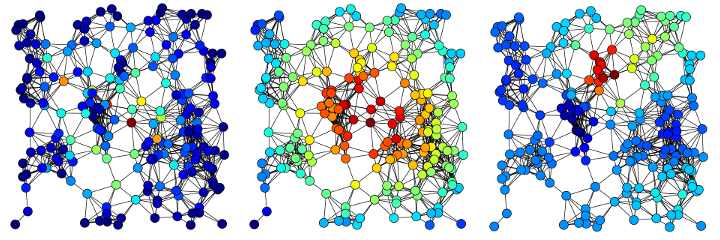
\includegraphics[width=\textwidth]{images/centrality.png}
                \caption{Examples of Betweenness centrality, Closeness centrality and Katz centrality of the same graph.}
                \label{centrality}
            \end{figure}
            
            For the moment, the function can use the following centrality measures: Betweenness, Closeness, Katz, Pagerank. However, it is easy to extend its functionality: other measures can be easily added.
            
            Here is a summary of what the function does and a description of its parameters and outputs.
            \begin{independentfunctiondoc}{most\_informative\_vertices}{graph, budget, centrality="pagerank"}
                \begin{functiondescription}
                    Find which are the most \textquote{important} vertices of the graph using a centrality measure.
                    
                    Once these vertices are labeled by the user, information is likely to propagate faster through the remaining vertices of the Wikipedia multilingual graph.
                \end{functiondescription}
                
                \begin{functionparameters}
                    \item[graph] \monospace{graph\_tool.Graph}
                    
                    Wikipedia graph.
                    
                    It can represent either a multilingual or a monolingual Wikipedia graph.
                    \item[budget] int
                    
                    Number of vertices to be returned.
                    \item[centrality] \{\inlinecode{"betweenness"}, \inlinecode{"closeness"}, \inlinecode{"katz"}, \inlinecode{"pagerank"}\}, default \inlinecode{"pagerank"}
                    
                    Centrality measure to be used for finding the most \textquote{important} vertices of the Wikipedia multilingual graph.
                \end{functionparameters}
                
                \begin{functionoutput}
                    Iterable object that contains the indexes of the most \textquote{important} vertices of the Wikipedia multilingual graph.
                    
                    Specifically, the returned iterable contains up to \normale{\emph{budget}} \normalfont indexes. Moreover, indexes are sorted by decreasing vertex desirability.
                \end{functionoutput}
            \end{independentfunctiondoc}
    \section{Curriculum}\label{curriculum}
        Following the idea of \citeauthor{Bengio} in \cite{Bengio}, the learning framework presented in this thesis allows to make use of \emph{curriculum learning}: inspired by how humans and animals seem to learn better, it is a type of learning in which at first the algorithm is presented simple examples, and then the difficulty of the tasks it has to solve gradually increases. For further details and a complete description of the approach, refer to section \ref{cv_learning}.
        
        Defining the curriculum is not an easy task, and general principles that make some strategies work better than others are still unknown. Indeed, it is difficult to define the notions of \textquote{easy} and \textquote{hard} instances. Moreover, it is not clear how much time the learner should spend on each difficulty level.
        
        Though there are still open questions around curriculum learning, it has showed good results in this setting (refer to section \ref{experiments_curricula} for more details):
        \begin{itemize}
            \item Models employing this technique are usually faster to train because time is not wasted in difficult tasks when the gained experience is not enough.
            \item Moreover, sometimes these algorithms seem to converge faster because they are guided towards better local minima.
        \end{itemize}
        Motivated by these promising results, I have decided to integrate curriculum learning into the framework and to provide users with:
        \begin{itemize}
            \item A function for defining an arbitrary curriculum --- i.e., a way for dividing the vertices of the Wikipedia multilingual graph into sets which are characterized by increasing difficulty or decreasing desirability.
            \item Some pre-defined functions for getting ready-to-use curricula and starting experimenting with curriculum learning.
        \end{itemize}
        \subsection{Load curriculum}
            The framework includes a function that allows to automatically load an arbitrary curriculum stored in a file. In this way, a user can define a curriculum, save it on disk for future reuse (computing a curriculum may be a computationally expensive operation: it is probably a bad idea to perform it twice) and load it whenever an experiment is done through the learning framework.
            
            The function works with CSV files: this means that data can be re-used also outside these specific settings.
            
            Here is a summary of what the function does and a complete description of parameters and outputs. The specific format of the CSV file will be described afterwards.
            \begin{independentfunctiondoc}{load\_curriculum}{graph, path}
                \begin{functiondescription}
                    Load curriculum from a CSV file.
                    
                    All the vertices which are not explicitly mapped to any difficulty level in the input CSV file are automatically assigned to an additional level that come after all the others.
                \end{functiondescription}
                
                \begin{functionparameters}
                    \item[graph] \monospace{graph\_tool.Graph}
                    
                    Wikipedia graph.
                    
                    It can represent either a multilingual or a monolingual Wikipedia graph. Refer to section \ref{categorygraphbuilder}, \ref{articlegraphbuilder} and \ref{multilingualbuilder} for checking how to build such specific graphs.
                    \item[path] string
                    
                    File path where the CSV file will be loaded.
                \end{functionparameters}
                
                \begin{functionoutput}
                    \monospace{graph\_tool.VertexPropertyMap} object, with associated value type \inlinecode{int}.
                    
                    This object provides a mapping from vertices of the graph to integer values. It is an external property: it is not memorized together with the graph and it does not need a name.
                \end{functionoutput}
            \end{independentfunctiondoc}
            \subsubsection{CSV file format}
                The CSV file from which curricula are loaded is formatted according to some standard basic rules:
                \begin{itemize}
                    \item It has no \textquote{header}.
                    \item Each line consists of exactly the same number of fields.
                    \item Values are separated by commas and are not quoted.
                    \item There are no leading and trailing spaces and/or tabs in any field.
                    \item Each line consists of a vertex index (a positive integer value) followed by one number representing the difficulty/desirability level the vertex belongs to (another positive integer value).
                \end{itemize}
                
                The CSV file where the curriculum is stored cannot contain more than one line for each vertex. This means that the number of lines of the CSV file must be less than or equal to the number of vertices in the Wikipedia graph, and that there must at most one occurrence of each vertex index. The specific order of lines does not matter.
                
                Moreover, if \(CV_{max}\) indicates the maximum difficulty level --- i.e., the last vertices on which the algorithm will be trained --- then the curriculum contained in the CSV file must map at least one vertex to each difficulty level included in the \(\left[0,CV_{max}\right]\) interval.
                
                Here is a practical example. Suppose that \inlinecode{graph} is an object of type \monospace{graph\_tool.Graph}. This graph has exactly ten nodes (with indexes going from \(0\) to \(9\)). This is a valid content for the \textquote{input.csv} file containing its curriculum:
                \begin{lstlisting}
2,1
0,3
5,2
7,0
                \end{lstlisting}
                All the nodes that are not explicitly mapped to any difficulty level are automatically assigned to an additional level:
                \begin{example}
// load curriculum
cv = load_curriculum(graph, "input.csv")
// get the difficulty level of the seventh vertex
v6 = graph.vertex(6)
v6_cv = cv[v6] // 4
                \end{example}
        \subsection{Predefined curricula}
            It is not easy to define the curriculum: it is not always clear how to create difficulty/desirability levels. However, a user can try out some of the ready-to-use curricula. Indeed, the framework provides users with two pre-defined functions that are able to compute meaningful curricula for a Wikipedia graph --- i.e., they partition vertices into several sets according to some notion of difficulty or desirability.
            \begin{enumerate}
                \item \monospace{article\_views\_curriculum} gives priority to vertices which correspond to highly visited pages. Intuitively, a page is more desirable if it has many visitors: one should pay more attention to such page.
                \item \monospace{merged\_vertices\_curriculum} gives priority to vertices which are the result of many merging operations between pages of different Wikipedia versions. Intuitively, a vertex which is shared between many different Wikipedia monolingual graphs is more important because once it is correctly labeled the information will propagate quickly to towards several different monolingual graphs.
            \end{enumerate}
            
            These functions always partition graph vertices into equally sized subsets. This is not necessarily the best choice one can make: sets corresponding to different difficulty/desirability levels could be unbalanced. For example, the basic level could comprise only few important vertices, while more advanced levels could have more. However, the main goal of this thesis is not to explore all the possible combinations of curricula, but to raise and study issues like this one and to provide some tools that allow easy experimentation. Therefore, curricula obtained through the use of these functions should be taken as a starting point for further experiments and trials.
            
            Here is a summary of what each function does and a complete description of parameters and outputs.
            \begin{independentfunctiondoc}{article\_views\_curriculum}{graph, levels}
                \begin{functiondescription}
                    Create a curriculum where vertices which correspond to pages with many visitors are assigned to early levels, and rarely visited vertices are left to last levels.
                    
                    Basically, this function sorts all the vertices of the Wikipedia multilingual graph by descending page views (vertices which have been merged are favored because their page views counters sum up) and partitions the set of vertices into equally sized subsets.
                \end{functiondescription}
                
                \begin{functionparameters}
                    \item[graph] \monospace{graph\_tool.Graph}
                    
                    Wikipedia multilingual graph.
                    \item[levels] int
                    
                    Number of subsets to partition the set of vertices.
                    
                    The number must be greater than 0.
                \end{functionparameters}
                
                \begin{functionoutput}
                    \monospace{graph\_tool.VertexPropertyMap} object, with associated value type \inlinecode{int}.
                    
                    This object provides a mapping from vertices of the graph to integer values. These values represent the curriculum level each vertex is assigned to.
                    
                    The returned object is an external property: it is not memorized together with the graph and it does not need a name.
                \end{functionoutput}
            \end{independentfunctiondoc}
            \begin{independentfunctiondoc}{merged\_vertices\_curriculum}{graph, levels}
                \begin{functiondescription}
                    Create a curriculum where vertices that are the result of many merging operations are assigned to early levels, and vertices that have few correspondences in other monolingual graphs are left to last levels.
                    
                    Basically, this function sorts all the vertices of the Wikipedia multilingual graph by descending number of IDs (vertices which have been merged many times are favored because they have more IDs than vertices which have undergone few merging operations) and partitions the set of vertices into equally sized subsets.
                \end{functiondescription}
                
                \begin{functionparameters}
                    \item[graph] \monospace{graph\_tool.Graph}
                    
                    Wikipedia multilingual graph.
                    \item[levels] int
                    
                    Number of subsets to partition the set of vertices.
                    
                    The number must be greater than 0.
                \end{functionparameters}
                
                \begin{functionoutput}
                    \monospace{graph\_tool.VertexPropertyMap} object, with associated value type \inlinecode{int}.
                    
                    This object provides a mapping from vertices of the graph to integer values. These values represent the curriculum level each vertex is assigned to.
                    
                    The returned object is an external property: it is not memorized together with the graph and it does not need a name.
                \end{functionoutput}
            \end{independentfunctiondoc}
    \section{Learning vertex embeddings}
        In this section I describe the machine learning algorithm that can be used to learn how to classify vertices of a Wikipedia multilingual graph. The function is very general and can be used to learn how to classify any graph. In particular, it has been designed to solve a semi-supervised problem (refer to section \ref{semi_supervised}) in which the graph is very large and only few vertex labels are know.
        
        Among other parameters, the function needs a generic graph, some labeled vertices, optional features and an optional curriculum. The format of these parameters is based on the generic classes \monospace{Graph} and \monospace{VertexPropertyMap} of the \monospace{graph\_tool} library: it does not depend on anything described in the previous sections. Indeed, chapter \ref{wikipedia_multilingual_graph} and sections \ref{features}, \ref{labels} and \ref{curriculum} simply describe some methods to build \monospace{graph\_tool.Graph} or \monospace{graph\_tool.VertexPropertyMap} instances. In particular, since all the objects and functions described in previous sections make use of the Builder design pattern, it is possible to separate the construction of complex objects from their representations, thus returning standard graphs and generic numerical properties defined on vertices.
        
        After an in-depth description of the generic framework, this section focuses on the implementation of some predefined components of the algorithm. Indeed, the framework is very general and can be used in many ways: if a user wants to quickly try it out on a Wikipedia multilingual graph then he/she can use one of the predefined implementations. In this way, one does not need to define a new machine learning model from scratch in order to be able to classify vertices of the graph.
        \subsection{Algorithm overview}\label{algorithm_overview}
            The proposed algorithm is mainly based on active learning (refer to section \ref{active_learning}): the main assumption is that it can achieve greater performance with less data if it is allowed to obtain the examples it desires and from which it learns. In other words, the cost of obtaining data is minimized by allowing the algorithm to decide which instances should be labeled in order to achieve a high accuracy.
            
            The algorithm is also based on curriculum learning (refer to section \ref{cv_learning}), in which the difficulty level of the training set is gradually increased: here, the main assumption is that being introduced to concepts by increasing complexity allows the learner to use previous experience to ease the learning of new concepts.
            
            Similarly to many different machine learning approaches, this algorithm is an iterative procedure that processes the entire training set at every epoch. Specifically, every iteration comprises:
            \begin{itemize}
                \item A training phase, in which the model is refined and its parameters tuned by using the vertices which belongs to a specific difficulty level of the training dataset.
                \item An evaluation phase, in which the model performance is evaluated using the vertices belonging to the evaluation dataset.
                \item An optional labelling phase, in which some of the unlabeled nodes belonging to the specific difficulty level of the training dataset are labeled through the use of an \textquote{oracle}. Labelling is not performed until a certain budget is reached\footnote{Most of the times, active learning algorithms are associated with a budget that must be respected.}.
            \end{itemize}
            At the end of the process, a test phase allows to assess the performance --- i.e., generalization --- of the final fully specified classifier.
            \begin{algorithm}
                \caption{Framework for learning vertex embeddings}
                \label{alg}
                \begin{algorithmic}[1] % The number tells where the line numbering should start
                    \Function{Learning-Framework}{$G$: graph, $F$: features, $L$: labels, $CV$: curriculum, $Tr$: training dataset, $Ev$: evaluation dataset, $Te$: test dataset, $trainer$: function defining how to process each epoch, $evaluator$: function defining how to evaluate the model, $tester$: function defining how to test the model, $oracle$: function defining how to label a vertex, $parameters$: function defining how to compute time-sensitive parameters, $EP$: epochs, $B$: budget, $batch$: batch size}
                        \State $\Phi_C \gets$ \Call{centrality}{$G$} \Comment{Compute centrality of each node}
                        \State $\mathcal{P}_C \gets$ Percentile of each centrality score
                        \State $time \gets 0$
                        \For{$level \in CV$}
                            \State $EP_{level} \gets$ Number of epochs for $level$
                            \State $B_{level} \gets$ Budget for $level$
                            \State $Tr_{level}^{(l)} \gets$ Labeled vertices in the training set and in $level$
                            \State $Tr_{level}^{(u)} \gets$ Unlabeled vertices in the training set and in $level$
                            \State $cost \gets 0$
                            \For{$i \in \left[1 \dots EP_{level}\right]$}
                                \State \Call{trainer}{$G, F, L, Tr_{level}^{(l)}$} \Comment{Process a training epoch}
                                \State $EM_{level}^i \gets$ Node embeddings
                                \State \Call{evaluator}{$G, F, L, Ev$} \Comment{Evaluate the model}
                                \If{$C < B_{level}$}
                                    \State $\Phi_D \gets$ \Call{density}{$EM_{level}^i$} \Comment{Compute density of each node}
                                    \State $\Phi_E \gets$ \Call{entropy}{$EM_{level}^i$} \Comment{Compute entropy of each node}
                                    \State $\mathcal{P}_D \gets$ Percentile of each density score
                                    \State $\mathcal{P}_E \gets$ Percentile of each entropy score
                                    \State $\alpha,\beta,\gamma \gets$ \Call{parameters}{$time$} \Comment{Time-sensitive parameters}
                                    \ForAll{$v \in Tr_{level}^{(u)}$}
                                        \State $S_v \gets \alpha \cdot \mathcal{P}_E(v) + \beta \cdot \mathcal{P}_D(v) + \gamma \cdot \mathcal{P}_C(v)$
                                    \EndFor
                                    \For{$j \in \left[1 \dots batch\right]$}
                                        \State $v_{best} \gets v \in Tr_{level}^{(u)}$ s.t. $S_v \ge S_w\  \forall w \in Tr_{level}^{(u)}$
                                        \State \Call{oracle}{$v_{best}$} \Comment{Label the best candidate}
                                        \State $Tr_{level}^{(u)} \gets Tr_{level}^{(u)} \setminus \left\{v_{best}\right\}$
                                        \State $Tr_{level}^{(l)} \gets Tr_{level}^{(l)} \cup \left\{v_{best}\right\}$
                                    \EndFor
                                    \State $cost \gets cost + batch$
                                \EndIf
                                \State $time \gets time + 1$
                            \EndFor
                        \EndFor
                        \State \Call{tester}{$G, F, L, Te$} \Comment{Test the model}
                    \EndFunction
                \end{algorithmic}
            \end{algorithm}
            
            Though the combination of active and curriculum learning makes this framework very flexible, what is really useful is how the query system work. In general, active learning algorithms that work on graphs need a query system that chooses a vertex and ask an oracle to label it. In this setting, a combination of different criteria is used (refer to section \ref{active_learning_criteria} for more details). Moreover, such combination of criteria depends on the state of the training: some criteria are preferred over the others depending on the current training epoch (refer to section \ref{combination_criteria}).
        \subsection{Signature}\label{signature}
            The function used to classify vertices of a graph is very flexible and can be highly customized by the user. In particular, before using the function, the user has to define a model to be used. After that, he/she has to tell the framework how to train, evaluate and test it. Then, the user has to specify how the \textquote{oracle} works --- i.e., which is the method used to answer the queries posed by the active learner.
            
            Moreover, the user can optionally specify other details, such as the curriculum and how to combine the different criteria used by the query system to find out the vertices to be labeled.
            
            All the specific details will be described later. Here the signature of the function is shown, together with a brief description of what each parameter is.
            \begin{independentfunctiondoc}{LF}{graph, features, labels, curriculum, train\_mask, eval\_mask, test\_mask, trainer, evaluator, tester, oracle, criteria\_parameters, epochs, budget=0, batch\_size=1}
                \begin{functiondescription}
                    Learn graph vertex embeddings --- i.e., learn how to classify vertices of a graph.
                    
                    This function can be used not only with Wikipedia multilingual graphs, but also with generic graphs.
                \end{functiondescription}
                
                \begin{functionparameters}
                    \item[graph] \monospace{graph\_tool.Graph}
                    
                    Generic graph.
                    
                    It can represent a Wikipedia multilingual graph built with functions presented in sections \ref{categorygraphbuilder}, \ref{articlegraphbuilder} and \ref{multilingualbuilder}.
                    \item[features] \monospace{graph\_tool.VertexPropertyMap}
                    
                    Object of type \monospace{graph\_tool.VertexPropertyMap} with associated value type \inlinecode{vector<double>}: it provides a mapping from vertices of \normale{\emph{graph}} \normalfont to arbitrary numerical features contained in a vector.
                    
                    Refer to section \ref{features} for more details on the creation of such object for the Wikipedia multilingual graph.
                    \item[labels] \monospace{graph\_tool.VertexPropertyMap}
                    
                    Object of type \monospace{graph\_tool.VertexPropertyMap} with associated value type \inlinecode{int}: it provides a mapping from vertices of \normale{\emph{graph}} \normalfont to integer labels.
                    
                    Refer to section \ref{labels} for more details on the creation of such object for the Wikipedia multilingual graph.
                    \item[curriculum] \monospace{graph\_tool.VertexPropertyMap}
                    
                    Object of type \monospace{graph\_tool.VertexPropertyMap} with associated value type \inlinecode{int}: it provides a mapping from vertices of \normale{\emph{graph}} \normalfont to integer difficulty levels.
                    
                    Refer to section \ref{curriculum} for more details on the creation of such object for the Wikipedia multilingual graph.
                    \item[train\_mask] \monospace{graph\_tool.VertexPropertyMap}
                    
                    Object of type \monospace{graph\_tool.VertexPropertyMap} with associated value type \inlinecode{boolean}: it provides a mapping from vertices of \normale{\emph{graph}} \normalfont to boolean values, which tell whether or not a vertex is part of the training dataset.
                    
                    All the unlabeled vertices of the graph must belong to the training set.
                    
                    Refer to section \ref{generalizability} for more details on the training dataset.
                    \item[eval\_mask] \monospace{graph\_tool.VertexPropertyMap}
                    
                    Object of type \monospace{graph\_tool.VertexPropertyMap} with associated value type \inlinecode{boolean}: it provides a mapping from vertices of \normale{\emph{graph}} \normalfont to boolean values, which tell whether or not a vertex is part of the evaluation dataset.
                    
                    An unlabeled vertex cannot be part of the evaluation dataset.
                    
                    Refer to section \ref{generalizability} for more details on the evaluation dataset.
                    \item[test\_mask] \monospace{graph\_tool.VertexPropertyMap}
                    
                    Object of type \monospace{graph\_tool.VertexPropertyMap} with associated value type \inlinecode{boolean}: it provides a mapping from vertices of \normale{\emph{graph}} \normalfont to boolean values, which tell whether or not a vertex is part of the test dataset.
                    
                    An unlabeled vertex cannot be part of the test dataset.
                    
                    Refer to section \ref{generalizability} for more details on the test dataset.
                    \item[trainer] function
                    
                    Function to be used for training the model.
                    
                    More details about the parameters and the output of this function are given is section \ref{train_eval_test_oracle}.
                    \item[evaluator] function
                    
                    Function to be used for evaluating the model.
                    
                    More details about the parameters and the output of this function are given is section \ref{train_eval_test_oracle}.
                    \item[tester] function
                    
                    Function to be used for testing the model once it is ready to use.
                    
                    More details about the parameters and the output of this function are given is section \ref{train_eval_test_oracle}.
                    \item[oracle] function
                    
                    Function to be used for labelling the vertices and answering the active learner queries.
                    
                    More details about the parameters and the output of this function are given is section \ref{train_eval_test_oracle}.
                    \item[criteria\_parameters] function
                    
                    Function used to compute the time-sensitive parameters used for combining the different query criteria (refer to sections \ref{active_learning_criteria} for more details).
                    
                    The function takes as input a single integer value which represents the current training epoch, and returns three values (\(\alpha\), \(\beta\) and \(\gamma\)). The returned values must sum up to \(1\).
                    
                    A possible implementation of such function is shown in section \ref{combination_criteria}.
                    \item[epochs] int or list of int
                    
                    Number of epochs --- i.e., how many times the algorithm has to iterate over all the vertices of the graph.
                    
                    When a curriculum comprises more than one difficulty/desirability level, a list of numbers can be specified in place of a single integer: each value corresponds to the number of epochs the algorithm will spend on each level.
                    \item[budget] int, default \inlinecode{0}
                    
                    Number of vertices that the oracle is able (or allowed) to label. Once the budget limit is reached, the active learner cannot query the oracle anymore.
                    \item[batch\_size] int, default \inlinecode{0}
                    
                    Number of queries the active learner is allowed to pose to the oracle at each epoch.
                \end{functionparameters}
                
                \begin{functionoutput}
                    \inlinecode{None}
                \end{functionoutput}
            \end{independentfunctiondoc}
        \subsection{Active learning criteria}\label{active_learning_criteria}
            In general, active learning algorithms that work on graphs need a query system that chooses a vertex and ask an oracle to label it. How to decide which instances are most informative and thus more desirable than others? Many strategies have been proposed. For example, a query system may label those instances that are most different from the current model, or in which disagreement among multiple classifiers is high etc.
            
            In this setting, I have decided to measure two different things: uncertainty and representativeness.
            \begin{enumerate}
                \item A model may be uncertain about the label to assign to a specific vertex. In general, the active learner should pick those vertices which the model is least certain with respect to classification prediction.
                \item Vertices which are good representations of the underlying data distribution are probably very important: one can search for representative vertices in the embedding space or in the graph structure itself. In general, the active learner should pick good representatives in order to make the information propagating faster.
            \end{enumerate}
            
            With regard to uncertainty, I have decided to measure it by using the information entropy:
            \[\Phi_E\left(v_i\right) = -\sum_{c}P_i^c \cdot log P_i^c\]
            where \(P_i^c\) is the probability that vertex \(v_i\) belongs to class \(c\), according to the current model. The larger \(\Phi_E\left(v_i\right)\) is, the more uncertain the current model is about the classification of \(v_i\).
            
            The problem of uncertainty measures is that noisy regions of the space might be found --- i.e., the active learner may start querying labels of unrepresentative vertices. To solve this problem, uncertainty measures can be combined with those based on representativeness: in this way, one can find representative vertices which the current model is uncertain about.
            
            I consider two representativeness measures: information density and graph centrality. The former aims to find a good representative vertex in the embedding space; the latter focuses on the centrality of a vertex in the graph.
            
            Density is measured as follow:
            \begin{enumerate}
                \item Apply the K-means clustering algorithm on the embeddings of unlabeled vertices.
                \item Compute the Euclidean distance between each embedding of a vertex and its cluster center.
                \item Compute the density score of each vertex by converting the distance value to a similarity score:
                \[\Phi_D\left(v_i\right) = \frac{1}{1+ED\left(Emb_{v_i},CC_{v_i}\right)}\]
                where \(ED\left(a,b\right)\) is the Euclidean distance between two points \(a\) and \(b\), \(Emb_{v_i}\) is the embedding of vertex \(v_i\) and \(CC_{v_i}\) is the center of the cluster \(v_i\) belongs to.
            \end{enumerate}
            
            With regard to the centrality, I have decided to measure it by using PageRank: it outperforms other measurements, as shown in \cite{Cai}. It is calculated as:
            \[\Phi_C\left(v_i\right) = \rho \sum_j A_{ij}\frac{\Phi_C\left(v_j\right)}{\sum_k A_{jk}} + \frac{1 - \rho}{N}\]
            where \(\rho\) is the damping parameter (usually roughly of order \(1\)), \(A\) is the adjacency matrix of the graph and \(N\) the number of vertices \cite{Newman}.
        \subsection{Combination of different criteria}\label{combination_criteria}
            In order to be able to choose the vertices that the oracle has to label, the three criteria presented in section \ref{active_learning_criteria} must be combined. There are two main issues to face:
            \begin{itemize}
                \item The scores given by different measurements are not comparable because they are on completely different scales. Combining them by simply using some scalar parameters is not a good idea because the results would be unpredictable and not meaningful.
                \item Certainly, the three criteria are all important, but some are more useful when the training has just begun, while others may be helpful only after many epochs. Specifically, \(\Phi_E\) and \(\Phi_D\) --- i.e., the entropy and density measurements --- are not very useful at the beginning: they rely on vertex embeddings, which are almost random when the training has just begun. On the other hand, \(\Phi_C\) --- i.e., graph centrality --- only relies on graph structure and therefore it could be helpful when there is no information about embeddings. As the training of the model advances, measurements related to embeddings should become more and more important, while those related to the graph structure should become less influential.
            \end{itemize}
            
            The first problem can be solved by normalizing scores and by turning them into percentiles as in \cite{Zhang}. Specifically, one can compute the percentile of unlabeled vertices which have a smaller score than vertex \(v_i\) in terms of metric \(\Phi\). Once the percentile scores have been computed, they can be linearly combined as:
            \[\alpha \cdot \mathcal{P}_E\left(v_i\right) + \beta \cdot \mathcal{P}_D\left(v_i\right) + \gamma \cdot \mathcal{P}_C\left(v_i\right)\]
            where \(\mathcal{P}_{\Phi}\left(v_i\right)\) represents the percentile of unlabeled vertices that have smaller metric \(\Phi\) than vertex \(v_i\), and where \(\alpha + \beta + \gamma = 1\). The goal is to find the unlabeled vertex belonging to the training set which maximizes the function: such vertex is at the same time a good representative of the underlying distribution and an instance the model is uncertain about.
            
            The second problem is strictly related to the definition of the parameters \(\alpha\), \(\beta\) and \(\gamma\): how can one choose these three parameters in a way that favourites centrality during the first epochs and entropy or density during the last ones? Here the problem is solved in the following way:
            \begin{enumerate}
                \item Find two parameters \(n_t^1\) and \(n_t^2\) whose value depends on time or, in other words, on the number of processed epochs. Specifically:
                \[n_t^1 = f\left(t\right)\]
                \[n_t^2 = g\left(t\right)\]
                where \(f\) is a non-negative increasing function of time and \(g\) is a non-negative decreasing function of time.
                \item Draw the parameters \(\alpha\) and \(\beta\) from a beta distribution with shape parameters \(1\) and \(n_t^2\). Draw the parameter \(\gamma\) from a beta distribution with shape parameters \(1\) and \(n_t^1\). In symbols:
                \[\alpha \sim Beta\left(1,n_t^2\right)\]
                \[\beta \sim Beta\left(1,n_t^2\right)\]
                \[\gamma \sim Beta\left(1,n_t^1\right)\]
                See figure \ref{beta_distribution} for an example.
                \item Divide each parameter by the sum of all the parameters, so that they sum up to \(1\), keeping at the same time their weights.
            \end{enumerate}
            
            \begin{figure}
                \centering
                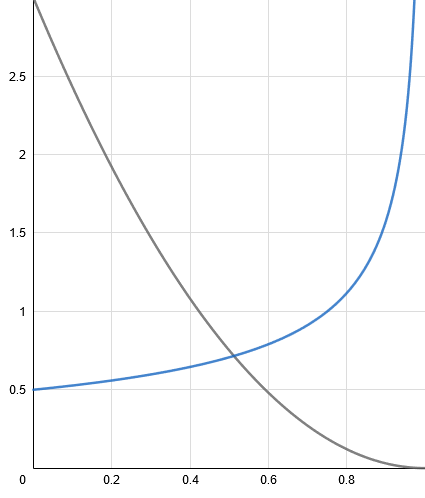
\includegraphics[width=0.5\textwidth]{images/beta.PNG}
                \caption{Examples of the probability density function for the Beta distribution \(Beta\left(\alpha,\beta\right)\). \(\alpha=1\) and \(\beta=3\) for the gray function. \(\alpha=1\) and \(\beta=0.5\) for the blue one.}
                \label{beta_distribution}
            \end{figure}
            Computing the parameters by drawing them from a probability distribution is usually better than computing them in a deterministic way, as shown in \cite{Cai}.
            
            Here is a possible implementation of a function that compute the three time-sensitive parameters:
            \begin{example}
def get_parameters(epoch):
    n1_t = log(epoch+1)+1
    n2_t = 1/n1_t
    parameters = np.array([np.random.beta(1, n2_t),
                           np.random.beta(1, n2_t),
                           np.random.beta(1, n1_t)])
    return parameters/np.sum(parameters)
            \end{example}
            In the example above, I have set \(f(t) = log(t+1)+1\) and \(g(t) = \frac{1}{log(t+1)+1}\).
        \subsection{Train, evaluate, test and label strategies}\label{train_eval_test_oracle}
            As described in section \ref{signature}, the functionality of the learning algorithm depends on three important functions: \monospace{trainer}, \monospace{evaluator} and \monospace{tester}. Through the definition of these functions, a user can customize the fundamental parts of the learning algorithm:
            \begin{itemize}
                \item At each epoch, the model has to be refined and its parameters tuned. The task of the \monospace{trainer} function is to define how this phase should be carried out. Specifically, it is responsible for finding the model that minimizes a certain loss function: this can be done by searching the parameter space. Refer to section \ref{components_ml} for more details.
                \item At each epoch, the current model can be evaluated by using the hold-out samples (refer to section \ref{validation}). Using the \monospace{evaluator} function, one can control whether the current model is over-fitting data or not.
                \item Finally, through the use of the \monospace{tester} function one can estimate the prediction error on new unseen data. This is done once the final model has been chosen. The measure obtained by using this function can be used as an estimator of the true error of the learned model.
            \end{itemize}
            
            These three functions share the same basic signature. Specifically, they take as input four parameters:
            \begin{parameters}
                \item[graph] \monospace{graph\_tool.Graph}
                
                Object that represents the domain structure.
                \item[features] \monospace{graph\_tool.VertexPropertyMap}
                
                Object that contains the features associated to each vertex of the graph (a mapping from vertices to \inlinecode{vector<double>} values).
                \item[labels] \monospace{graph\_tool.VertexPropertyMap}
                
                Object that contains the labels associated to each vertex of the graph (a mapping from vertices to \inlinecode{int} values).
                \item[vertices\_mask] \monospace{graph\_tool.VertexPropertyMap}
                
                Mask that defines which vertices can be used by the function (a mapping from vertices to \inlinecode{Bololean} values).
            \end{parameters}
            In particular, the \monospace{trainer} function can use only unlabeled training vertices belonging to a certain difficulty level of the curriculum; \monospace{evaluator} and \monospace{tester} use, respectively, the evaluation and test dataset.
            
            Besides \monospace{trainer}, \monospace{evaluator} and \monospace{tester}, there is another important function that can be customized by the user, and it differentiates this framework from many others: \monospace{oracle} defines how some arbitrary chosen unlabeled vertices (refer to sections \ref{active_learning_criteria} and \ref{combination_criteria}) can be labeled --- i.e., it specifies how the queries posed by the active learned should be answered. In other words, the query system find unlabeled vertices whose labels are very desirable; these vertices are then processed through the \monospace{oracle} function, which must return a label for each of them (this can be done by asking a user to input a label, by using an automatic algorithm, or by querying an external database, etc.).
            
            The \monospace{oracle} function takes as input two parameters:
            \begin{parameters}
                \item[graph] \monospace{graph\_tool.Graph}
                
                Object that represents the domain structure.
                \item[vertices] iterable of \monospace{graph\_tool.Vertex}
                
                Iterable containing all the vertices of the graph that should be labeled by the \monospace{oracle} function (for more details on the \monospace{graph\_tool.Vertex} class refer to \url{https://graph-tool.skewed.de/static/doc/graph_tool.html#graph_tool.Vertex}).
            \end{parameters}
            
            The \monospace{oracle} function returns an iterable of \inlinecode{int} values, each representing a hard label corresponding to the related input vertex. Alternatively, if one wants to provide more accurate label information to the algorithm, the \monospace{oracle} function can return an iterable of \inlinecode{vector<doubles>} (where the values are all positive and sum up to \(1\)), each representing a soft label corresponding to the related vertex. In general, if one plans to label many vertices at the same time then he/she should consider to return a generator instead of a list.
            
            Refer to section \ref{algorithm_overview} for a complete overview of the algorithm and to check how these four functions are used in its context.
        \subsection{Querying the labelling platform}
            Chapter \ref{labelling_platform} describes a labelling platform that can be used to collect the labels associated to arbitrary Wikipedia pages. Specifically, section \ref{rest_api} describes the REST-based APIs provided by the platform.
            
            I have decided to implement an oracle function --- \monospace{labelling\_platform\_oracle} --- that makes use of these services provided by the labelling platform. In particular, this function queries the platform to understand whether it already contains the desired data; if this is not the case, the function posts new data on the platform database and waits until a user gives an answer.
            
            The uploaded data are prioritized so that they are processed as soon as possible. Moreover, the function is implemented through the use of a generator, therefore the learning algorithm does not have to wait for the entire list to be ready, but can continue its execution every time a label is received. Finally, a timer checks when time is out: when the platform does not provide an answer within a certain time, the oracle stop waiting and let the training of the model continue.